\documentclass[11pt]{article}
\usepackage{iftex}
\ifPDFTeX
  \pdfinfoomitdate=1
  \pdftrailerid{}
  \pdfsuppressptexinfo=15
\fi
\usepackage[margin=0.86in]{geometry}
\usepackage{amsmath,amssymb,amsthm,mathtools}
\usepackage{booktabs,array,longtable}
\usepackage{enumitem}
\usepackage{xcolor}
\usepackage{microtype}
\usepackage{tikz}
\usetikzlibrary{arrows.meta,positioning,calc}
\usepackage[hidelinks]{hyperref}
\usepackage[nameinlink,noabbrev]{cleveref}
\usepackage{fancyhdr}
\usepackage{lastpage}

\definecolor{navy}{HTML}{17365D}
\definecolor{lightblue}{HTML}{EAF2F8}

\newtheorem{theorem}{Theorem}[section]
\newtheorem{lemma}[theorem]{Lemma}
\newtheorem{proposition}[theorem]{Proposition}
\newtheorem{corollary}[theorem]{Corollary}
\theoremstyle{remark}
\newtheorem{remark}[theorem]{Remark}

\newcommand{\R}{\mathbb{R}}
\newcommand{\one}{\mathbf{1}}
\newcommand{\cond}{\operatorname{cond}}
\newcommand{\good}{\mathcal{G}}
\newcommand{\bad}{\mathcal{B}}
\newcommand{\K}{\mathcal{K}}
\newcommand{\eps}{\varepsilon}

\pagestyle{fancy}
\fancyhf{}
\lhead{Fixed-Gadget Scenario-Cover Program}
\rhead{v0.3.0 -- unrefereed research release}
\cfoot{\thepage\ of \pageref{LastPage}}
\setlength{\headheight}{14pt}

\title{\textbf{Scenario-Cover Geometry for a Four-Terminal\\
Planar Unsplittable-Flow Gadget}\\[5pt]
\large Integrated technical synopsis with companion proofs}
\author{Matthew Protti}
\date{4 August 2026}

\begin{document}
\maketitle

\begin{center}
\fcolorbox{navy}{lightblue}{\parbox{0.91\textwidth}{\small
\textbf{Scope and status.}
This technical synopsis integrates a fixed-gadget theorem program supported by
versioned evidence and complete companion proofs in the v0.3.0 repository.
It is not an unrestricted planar-SSUF theorem, complete external human review,
conventional journal peer review, proof-assistant verification, or exhaustive
novelty clearance.
The controlling one-scenario, repaired high-$\kappa$, and frozen review sources
have been authenticated. R4 v6 accepted the cross-package scope statements,
while the separate publication decision was made by the named human author.
One supplied external human report reconstructed
the duality and short GM-005/006 arguments but did not inspect the full SC-006
or GM-008/009 proofs; it is scope-limited, not full acceptance. This synopsis
is not a standalone substitute for its companion proof artifacts. No license
is granted by this release.}}
\end{center}

\begin{abstract}
We study a fixed planar acyclic single-source unsplittable-flow gadget with four
terminals and two designated source--terminal paths per terminal. For strictly
positive full-demand route-cost-difference scenarios, the following
fixed-gadget scenario-count ladder is supported by complete analytic proof
sources and narrower exact corroboration:
\[
\beta_G^{(m,+)}=
\begin{cases}
(299-41\sqrt{41})/32,&m=1,\\
17/8,&m=2,\\
3,&m=3,\\
4,&m\ge4.
\end{cases}
\]
The two-, three-, and four-or-more-scenario suprema are not attained by finite
legal instances. No attainment or nonattainment assertion is made for the
one-scenario supremum. The one-scenario value also holds for the broader class of
legally realizable signed and zero route-cost differences, but no such
multi-scenario extension is claimed.

The $m=1$ equality in this integrated ladder is the later GM-002/003
arbitrary/legal fixed-gadget theorem. The immutable public v0.1.0/v0.2.1
one-scenario disclosure proves the same radical for its narrower lower family;
the two statements must not be conflated.

The organizing principle is exact scenario-cover duality: to force all common
cost-nonincreasing routings above a deviation threshold, the scenarios' open
homogeneous halfspaces must cover every lower-deviation routing displacement.
At one rational RB witness, an exact atlas classifies all 168 downsets of the
four-cube, 59 realizable positive-scenario losing patterns, 32
condition-number infima, and every one- through four-scenario cover count.
A separately isolated blind implementation reproduced the fixed finite
mathematical data after lossless convention normalization; strict certificate
payloads were not identical, and that distinction is retained.

For the RB family
$p_\eps=(1/4+\eps,\eps,1/2,1/4+\eps)$,
$d=(1,1,3/4,1)$, we give an exact four-phase two-scenario condition-number
diagram. The repaired global fixed-gadget theorem gives
$\beta_G^{(2,+)}(\kappa)\le2$ for $1\le\kappa\le2$; for $\kappa>2$ it gives
$\beta_G^{(2,+)}(\kappa)\le\max\{2,F(\kappa)\}$, with exact equality to
$F(\kappa)$ for $\kappa\ge\kappa_0$, where $\kappa_0$ is the largest real
root of an explicit quartic. The exact middle curve below $\kappa_0$ remains
open.
\end{abstract}

\tableofcontents
\newpage

\section{The fixed gadget and robust objective}

The graph is the released four-terminal planar DAG. It has a five-arc trunk
$a_1,\ldots,a_5$, and each terminal $i\in[4]$ has an E path and a C path.
Relative to the E path, switching terminal $i$ to its C path adds its full
demand on the trunk support
\[
I_1=\{a_1,a_2,a_3\},\quad
I_2=\{a_1,a_2,a_3,a_4,a_5\},\quad
I_3=\{a_2,a_3,a_4,a_5\},\quad
I_4=\{a_3,a_4\}.
\tag{1.1}
\]
There are also two private arcs per terminal, so every candidate routing is
checked on thirteen arcs.

\begin{figure}[ht]
\centering
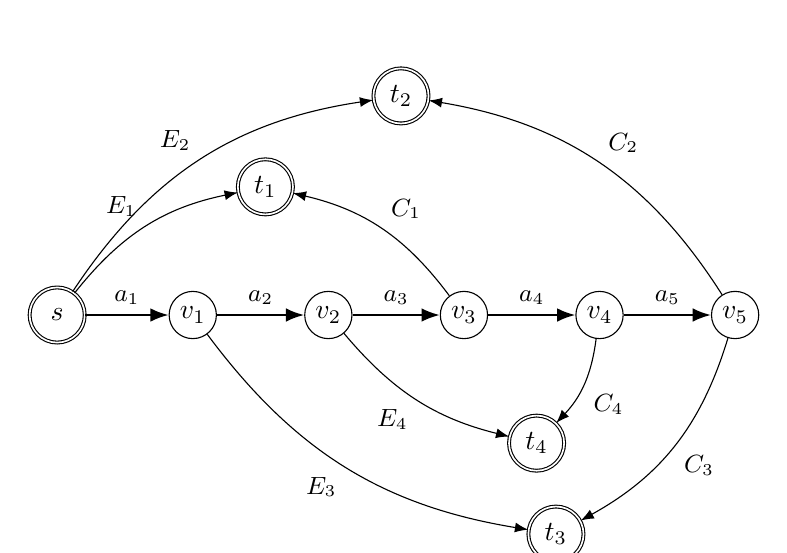
\begin{tikzpicture}[x=1.23cm,y=1.05cm,>=Latex,
  trunk/.style={->,thick}, branch/.style={->,thin},
  node/.style={circle,draw,fill=white,minimum size=6mm,inner sep=0pt},
  terminal/.style={double,circle,draw,fill=white,minimum size=7mm,inner sep=0pt},
  lab/.style={font=\small}]
\node[terminal] (s) at (0,0) {$s$};
\node[node] (v1) at (1.4,0) {$v_1$};
\node[node] (v2) at (2.8,0) {$v_2$};
\node[node] (v3) at (4.2,0) {$v_3$};
\node[node] (v4) at (5.6,0) {$v_4$};
\node[node] (v5) at (7.0,0) {$v_5$};
\draw[trunk] (s)--node[above,lab]{$a_1$}(v1);
\draw[trunk] (v1)--node[above,lab]{$a_2$}(v2);
\draw[trunk] (v2)--node[above,lab]{$a_3$}(v3);
\draw[trunk] (v3)--node[above,lab]{$a_4$}(v4);
\draw[trunk] (v4)--node[above,lab]{$a_5$}(v5);
\node[terminal] (t1) at (2.15,1.55) {$t_1$};
\node[terminal] (t2) at (3.55,2.65) {$t_2$};
\node[terminal] (t4) at (4.95,-1.55) {$t_4$};
\node[terminal] (t3) at (5.15,-2.65) {$t_3$};
\draw[branch,bend left=20] (s) to node[above left,lab]{$E_1$} (t1);
\draw[branch,bend right=20] (v3) to node[above right,lab]{$C_1$} (t1);
\draw[branch,bend left=24] (s) to node[above left,lab]{$E_2$} (t2);
\draw[branch,bend right=24] (v5) to node[above right,lab]{$C_2$} (t2);
\draw[branch,bend right=22] (v1) to node[below left,lab]{$E_3$} (t3);
\draw[branch,bend left=22] (v5) to node[below right,lab]{$C_3$} (t3);
\draw[branch,bend right=18] (v2) to node[below left,lab]{$E_4$} (t4);
\draw[branch,bend left=18] (v4) to node[below right,lab]{$C_4$} (t4);
\end{tikzpicture}
\caption{Schematic of the released two-path gadget. The proof uses the
path-difference supports in (1.1); private arcs permit legal realization of
full-demand route-cost differences.}
\label{fig:gadget}
\end{figure}

Let $0<d_i\le1$ and normalize $d_{\max}=1$. Let $p_i\in[0,1]$ be the
fractional C fraction and
let $S\subseteq[4]$ be the C-set of an unsplittable routing. Write
\[
v_S:=\one_S-p\in\R^4.
\tag{1.2}
\]
For a full-demand E-minus-C route-cost-difference vector $k$,
\[
c(y^S)-c(x)=k\cdot p-k(S)=-k\cdot v_S.
\tag{1.3}
\]
Thus $S$ is cost-nonincreasing exactly when
\[
k\cdot v_S\ge0.
\tag{1.4}
\]
Every positive $k$ is physically realizable using nonnegative,
commodity-independent arc costs: place cost $k_i/d_i$ on an E-private arc of
terminal $i$ and zero on the corresponding C-private arc and all other arcs.

Let $M(S;p,d)$ be the maximum positive deviation of route $S$ from the
fractional flow over all thirteen arcs.
For a trunk arc $a$, direct path-incidence subtraction gives
\[
\Delta_a(S)=
\sum_{\substack{i\in S\\a\in I_i}}h_i
-\sum_{\substack{i\notin S\\a\in I_i}}\ell_i,
\qquad
h_i=d_i(1-p_i),\quad \ell_i=d_ip_i,
\tag{1.4a}
\]
where $S$ is the C-set. Thus
\[
M(S;p,d)\le
\max\left\{1,\sum_{i\in S}h_i\right\}
\le\max\{1,|S|\}.
\tag{1.4b}
\]
The first term covers all eight terminal-private arcs: each positive private
deviation is either $h_i$ or $\ell_i$, hence at most $d_i\le1$. Equations
(1.4a)--(1.4b) are proved without enumeration in the companion
\path{research/fixed_gadget_scenario_cover/scenario_ladder/TRUNK_PRIVATE_ARC_ENVELOPE.md}
and structurally checked for all sixteen routings by its exact verifier.

For positive scenarios $k^{(1)},\ldots,k^{(m)}$, define
\[
\Phi(p,d;k^{(1)},\ldots,k^{(m)})
:=\min_{\substack{S\subseteq[4]\\k^{(j)}\cdot v_S\ge0\ \forall j}}
M(S;p,d).
\tag{1.5}
\]
The feasible family is nonempty: the all-C C-set $[4]$ has displacement
$\one-p\ge0$ and is feasible in every positive scenario.
Let $\beta_G^{(m,+)}$ be the supremum of (1.5) over legal normalized data
on this fixed gadget.

Some proofs are shorter in the E-set orientation $R=[4]\setminus S$. Put
$q=\one-p$. Then $R$ is feasible in a positive scenario exactly when
\[
k(R)\le k\cdot q.
\tag{1.6}
\]

\section{Scenario-cover duality}

For one positive scenario define the eliminated downset
\[
\bad(k;p):=\{S\subseteq[4]:k\cdot v_S<0\}.
\tag{2.1}
\]
For a target deviation $t$, define
\[
\good_{<t}(p,d):=\{S\subseteq[4]:M(S;p,d)<t\}.
\tag{2.2}
\]
Strictness is essential: a route tying a scenario budget is feasible, and a
route tying $t$ need not be eliminated to force value at least $t$.

\begin{theorem}[Exact scenario-cover duality]\label{thm:duality}
For positive scenarios $k^{(1)},\ldots,k^{(m)}$,
\[
\Phi(p,d;k^{(1)},\ldots,k^{(m)})\ge t
\quad\Longleftrightarrow\quad
\good_{<t}(p,d)\subseteq\bigcup_{j=1}^m\bad(k^{(j)};p).
\tag{2.3}
\]
\end{theorem}

\begin{proof}
The left side says that no common feasible routing has deviation below $t$.
By (1.4), a route is not common feasible exactly when at least one scenario
has negative dot product with its displacement. This is precisely the cover
statement on the right.
\end{proof}

For $\kappa\ge1$, let
\[
\K_\kappa:=\left\{k\in\R^4_{>0}:
\frac{\max_i k_i}{\min_i k_i}\le\kappa\right\}.
\tag{2.4}
\]
For a route family $\mathcal A$, define
\[
\tau_{\kappa,p}(\mathcal A):=
\min\left\{m:\mathcal A\subseteq\bigcup_{j=1}^m\bad(k^{(j)};p),
\ k^{(j)}\in\K_\kappa\right\}.
\tag{2.5}
\]
Use $\tau_{\kappa,p}(\varnothing)=0$ and value $+\infty$ when no cover exists;
$\kappa=\infty$ means unrestricted positive normals. A cover with fewer than
$m$ scenarios may be padded by duplicating a positive scenario, so exact and
at-most conventions agree for the value. Cover thresholds are infima and
strict endpoint availability is checked separately.
If $\mathcal R(p,d)$ is the finite set of route values,
\[
\Psi_{m,\kappa}(p,d)=
\max\left\{r\in\mathcal R(p,d):
\tau_{\kappa,p}(\good_{<r}(p,d))\le m\right\}.
\tag{2.6}
\]
Locally, $\beta_G^{(m,+)}(\kappa)$ denotes the supremum of (2.6) over
$p\in[0,1]^4$ and positive normalized $d$ on this fixed gadget.
Multi-scenario robust rounding is therefore a restricted open-halfspace cover
problem on sixteen routing displacement vectors.

\section{The fixed-gadget scenario-count ladder}

Let
\[
L:=\frac{299-41\sqrt{41}}{32}=1.139747070789\ldots.
\tag{3.1}
\]
The integrated v0.3.0 claim ledger is
\[
\boxed{
\beta_G^{(m,+)}=
\begin{cases}
L,&m=1,\\
17/8,&m=2,\\
3,&m=3,\\
4,&m\ge4.
\end{cases}}
\tag{3.2}
\]
The evidence is modular. R1 v2 accepted GM-002 and GM-003 at claim level while
its packet retained editorial repairs; the complete derived one-scenario proof
and pinned dependencies are companion artifacts under
\texttt{research/fixed\_gadget\_scenario\_cover/one\_scenario/}. The $m=2$
proof remains the immutable unrefereed v0.2.1 RB-003 package. R2 v2 accepted
the repaired GM-005 proof, and original R2 accepted GM-006 at claim level. The
complete current GM-005 and GM-006 proofs are companion artifacts under
\texttt{scenario\_ladder/}; the short arguments below are their synopsis.
The complete, hash-bound reviewer index is
\path{research/fixed_gadget_scenario_cover/FULL_PROOF_REVIEW_MAP.md}.

\subsection{Three positive scenarios}

Use the E-set orientation and put
\[
h_i=d_iq_i,\qquad H=\sum_i h_i.
\tag{3.3}
\]
The all-C route is always feasible and has exact value $H$.

\begin{lemma}[Singleton assignment]\label{lem:assign}
If every singleton E-set is blocked by at least one of three positive
scenarios, then $H<3$.
\end{lemma}

\begin{proof}
If $q=0$, then $H=0<3$. Otherwise set
$B_j=k^{(j)}\cdot q>0$ and $w^{(j)}=k^{(j)}/B_j$, so
$w^{(j)}\cdot q=1$. Assign each singleton to one scenario that blocks it, with
assigned group $G_j$. Blocking is strict, so $w_i^{(j)}>1$ for $i\in G_j$.
For a positive-mass group,
\[
\sum_{i\in G_j}h_i
<\sum_{i\in G_j}h_iw_i^{(j)}
\le\sum_iq_iw_i^{(j)}=1,
\tag{3.4}
\]
because $h_i=d_iq_i\le q_i$. Empty or zero-mass groups contribute $0<1$.
Summing gives $H<3$.
\end{proof}

\begin{lemma}[Equality collapse]\label{lem:collapse}
If some singleton E-set $\{r\}$ is feasible, the instance has a feasible
routing of value strictly below three.
\end{lemma}

\begin{proof}
The singleton route has at most three positive C-terminal contributions on
any trunk, each at most one, and private deviation at most one. Its value is
therefore at most three. Equality forces $h_i=d_iq_i=1$ for every $i\ne r$,
hence $d_i=q_i=1$ for those three terminals. The complementary E-triple
$T=[4]\setminus\{r\}$ is feasible in every scenario because
\[
k^{(j)}(T)=\sum_{i\ne r}k_i^{(j)}
=\sum_{i\ne r}q_ik_i^{(j)}\le k^{(j)}\cdot q.
\tag{3.5}
\]
In route $T$, the three E-routed terminals have
$d_i(1-q_i)=0$; only terminal $r$ can contribute positively, so the route has
value at most one.
\end{proof}

\begin{theorem}[Three-scenario branch]\label{thm:m3}
$\beta_G^{(3,+)}=3$, and every finite legal instance has value strictly below
three.
\end{theorem}

\begin{proof}
Either all singletons are blocked and \cref{lem:assign} gives the all-C route
value $H<3$, or a singleton is feasible and \cref{lem:collapse} gives a route
below three. For the lower sequence, take an integer $n\ge2$, unit demands,
$q_i=1-1/n$, and
\[
(3n,1,1,1),\quad(1,3n,1,1),\quad(1,1,3n,1).
\tag{3.6}
\]
The common feasible E-sets are exactly $\varnothing$ and $\{4\}$. The latter
route has exact value $3(1-1/n)\to3$.
\end{proof}

\subsection{Four or more positive scenarios}

\begin{theorem}[Many-scenario branch]\label{thm:m4}
For every integer $m\ge4$, $\beta_G^{(m,+)}=4$, and every finite legal
instance has value strictly below four.
\end{theorem}

\begin{proof}
The all-C route has value $H=\sum_i d_iq_i\le4$. For an integer $n\ge2$,
unit demands, and $q_i=1-1/n$, use
\[
(3n,1,1,1),\quad(1,3n,1,1),\quad
(1,1,3n,1),\quad(1,1,1,3n).
\tag{3.7}
\]
Every nonempty E-set is blocked by a scenario heavy on one of its terminals,
so only $\varnothing$ is common feasible, with value $4(1-1/n)\to4$. Repeat a
scenario for $m>4$.

If a finite instance had value four, the all-C route would force
$d_i=q_i=1$ for all $i$. The full E-set would then be weakly feasible at
equality in every scenario and would have zero deviation, a contradiction.
\end{proof}

\begin{remark}
The $m=2$, $m=3$, and $m\ge4$ values are nonattained. GM-002 is a
supremum-only statement; this synopsis asserts neither attainment nor
nonattainment for $m=1$.
\end{remark}

\section{Exact finite scenario-cover atlas}

At the rational RB witness
\[
p=\left(\frac{251}{1000},\frac1{1000},\frac12,
\frac{251}{1000}\right),\qquad
d=\left(1,1,\frac34,1\right),
\tag{4.1}
\]
the sixteen route levels are as follows.

\begin{table}[ht]
\centering
\caption{Exact route values at the finite RB witness.}
\label{tab:routes}
\begin{tabular}{@{}lc@{}}
\toprule
C-set(s) & $M(S;p,d)$\\
\midrule
$\varnothing,3$ & $3/8$\\
$1,4$ & $749/1000$\\
$2$ & $999/1000$\\
$14$ & $561/500$\\
$13,34$ & $1123/1000$\\
$24$ & $1373/1000$\\
$23$ & $687/500$\\
$12$ & $437/250$\\
$134$ & $234/125$\\
$124$ & $1061/500$\\
$123,234$ & $2123/1000$\\
$1234$ & $359/125$\\
\bottomrule
\end{tabular}
\end{table}

The exact atlas classifies all 168 downsets of the four-cube. Exactly 59 are
one-scenario losing families at this $p$, with 32 distinct condition-number
infima. Minimum cover counts are
\[
\begin{array}{c|rrrrrr}
\text{cover count}&0&1&2&3&4&\text{impossible}\\\hline
\text{downsets}&1&61&91&13&1&1.
\end{array}
\tag{4.2}
\]
The unique four-scenario downset is all proper C-sets; the full cube is
impossible because all-C cannot be eliminated by a positive scenario.

With unrestricted positive normals, the fixed point has
\[
\begin{array}{c|cccc}
m&1&2&3&4\\\hline
\Psi_{m,\infty}(p,d)&561/500&1061/500&2123/1000&359/125.
\end{array}
\tag{4.3}
\]
These are fixed-instance encoded values, not the global fixed-gadget values in
(3.2). The checkers do not certify unencoded orientation, analytic case
exhaustion, global optimization, dependency correctness, statement scope,
novelty, authorship, or rights.

For two scenarios, set
\[
A=\frac{1498}{501},\qquad B=998,\qquad C=1998.
\tag{4.4}
\]
Then
\[
\Psi_{2,\kappa}(p,d)=
\begin{cases}
561/500,&1\le\kappa\le A,\\
1123/1000,&A<\kappa\le B,\\
234/125,&B<\kappa\le C,\\
1061/500,&C<\kappa.
\end{cases}
\tag{4.5}
\]
Each new phase starts strictly after its breakpoint.

\subsection{Blind finite reconstruction}

R3B v2 was developed under technically enforced answer isolation, frozen
before expected outputs and comparison code were disclosed, and returned
\texttt{ACCEPT\_AS\_STATED}. For all 451 compared certificates, the primal and
objective magnitude agreed, and both certificate populations exact-validated after lossless
convention projection. Fourteen degenerate LPs used alternative valid duals.

The raw strict-payload comparator nevertheless returned \texttt{FAIL}.
The correct label is
\[
\boxed{\texttt{SEMANTIC\_MATHEMATICAL\_MATCH}\ /\ 
\texttt{STRICT\_CERTIFICATE\_PAYLOAD\_IDENTITY\_FAIL}.}
\tag{4.6}
\]
Thus \texttt{BLIND\_INDEPENDENT\_REPRODUCTION} applies only to this fixed
finite atlas.

\section{Exact RB-family two-scenario phase}

For $0<\eps<1/8$, set
\[
p_\eps=\left(\frac14+\eps,\eps,\frac12,\frac14+\eps\right),
\qquad d=\left(1,1,\frac34,1\right),
\tag{5.1}
\]
and
\[
A(\eps)=\frac{3-4\eps}{1+2\eps},\qquad
B(\eps)=\frac1\eps-2,\qquad
C(\eps)=\frac2\eps-2.
\tag{5.2}
\]
Put
\[
r_0=\frac98-3\eps,\quad
r_1=\frac98-2\eps,\quad
r_2=\frac{15}{8}-3\eps,\quad
r_3=\frac{17}{8}-3\eps.
\tag{5.3}
\]

\begin{theorem}[SC-006]\label{thm:sc006}
For exactly two positive scenarios of condition number at most $\kappa$,
\[
\Psi_{2,\kappa}(p_\eps,d)=
\begin{cases}
r_0,&1\le\kappa\le A(\eps),\\
r_1,&A(\eps)<\kappa\le B(\eps),\\
r_2,&B(\eps)<\kappa\le C(\eps),\\
r_3,&C(\eps)<\kappa.
\end{cases}
\tag{5.4}
\]
Every breakpoint belongs to the lower branch.
\end{theorem}

The first transition is controlled by route $14$:
\[
T(1,\kappa,\kappa,1)-k(14)
=\left(\frac12+\eps\right)(\kappa-A(\eps)),
\tag{5.5}
\]
with a matching upper inequality for every $\kappa$-bounded scenario.

For the middle transition, if one scenario eliminates any two of the outer
pairs $13,14,34$, adding the strict losing inequalities gives
\[
\cond(k)>\frac{1-2\eps}{\eps}=B(\eps).
\tag{5.6}
\]
Two scenarios covering three outer pairs therefore force one across $B$.
Above $B$, the star--triangle normals
\[
(1,\kappa,1,1),\qquad(\kappa,1,\kappa,\kappa)
\tag{5.7}
\]
cover all six pairs.

The third transition is controlled by route $134$:
\[
T(k)-k(134)\le\eps(\kappa-C(\eps))\min_i k_i.
\tag{5.8}
\]
Above $C$, the first normal in (5.7) also eliminates $134$.

Finally, one scenario cannot eliminate both triples $134$ and $124$.
A scenario eliminating $134$ accepts every set containing terminal 2, while a
scenario eliminating $124$ accepts every set containing terminal 3. Two
scenarios assigned one triple each therefore both accept $23$. This proves
the unrestricted fixed-family ceiling $r_3$.

The endpoint $\eps=1/8$ is excluded because the route filtration changes.
SC-006 is fixed-family, exactly-two-scenario, and positive-coordinate only.
The complete reviewed proof is the companion artifact
\texttt{scenario\_cover/SC006\_CONTINUUM\_THEOREM.md}; this section is a
synopsis rather than a replacement for that proof.

\section{High-heterogeneity global tail}

Define
\[
F(\kappa)=
\frac{17\kappa^4-22\kappa^3-13\kappa^2+18\kappa+1}
{8(\kappa^2-1)^2},
\tag{6.1}
\]
and let $\kappa_0$ be the largest real root of
\[
P(\kappa)=\kappa^4-22\kappa^3+19\kappa^2+18\kappa-15.
\tag{6.2}
\]
Then
\[
\kappa_0=21.058780922898283\ldots,\qquad F(\kappa_0)=2.
\tag{6.3}
\]

\begin{theorem}[Internally reviewed high-$\kappa$ tail and global bounds]
For the fixed gadget and exactly two positive scenarios,
\[
L\le\beta_G^{(2,+)}(\kappa)\le2\qquad(1\le\kappa\le2),
\]
\[
\max\{L,F(\kappa)\}\le\beta_G^{(2,+)}(\kappa)\le2
\qquad(2<\kappa<\kappa_0),
\]
and
\[
\boxed{\beta_G^{(2,+)}(\kappa)=F(\kappa)
\qquad(\kappa\ge\kappa_0).}
\tag{6.4}
\]
\end{theorem}

The cover geometry explains the parameters. If $Q$ is the central E fraction
and $S$ the total outer E fraction, the center-heavy and outer-heavy cover
boundaries are
\[
S=\kappa(1-Q),\qquad S=2-\frac{Q}{\kappa}.
\tag{6.5}
\]
Their intersection is
\[
Q_\kappa=\frac{\kappa(\kappa-2)}{\kappa^2-1},\qquad
S_\kappa=\frac{\kappa(2\kappa-1)}{\kappa^2-1}.
\tag{6.6}
\]
Substitution into the accepted load envelope gives
$F(\kappa)=Q_\kappa+(1+S_\kappa)^2/8$, and
\[
F(\kappa)-2=
\frac{P(\kappa)}{8(\kappa-1)^2(\kappa+1)^2}.
\tag{6.7}
\]
The complete companion proof is
\texttt{bounded\_heterogeneity/GM008\_GM009\_HIGH\_KAPPA\_THEOREM.md}. It
contains the RB-003 value-above-two branch reduction, strict star and triangle
inequalities, the early $t\le2$ split, exact three-regime allocation envelope,
one-variable maximization, strict lower family, and quartic-root argument. In
particular, a feasible outer singleton first gives
$t\le\max\{1,H-h_i\}$; only the standing $t>2$ branch yields
$t\le H-h_i$. The exact curve on $1\le\kappa<\kappa_0$ remains open; the upper
bound by two is not an equality classification. No claim of finite attainment
for $F(\kappa)$ is made here.

\section{Related and concurrent work}

The primary records were checked on 2 August 2026. Sergey Nikolenko's first
manuscript is dated 29 July 2026 and its Zenodo record was published 30 July
2026 (DOI \href{https://doi.org/10.5281/zenodo.21701162}%
{10.5281/zenodo.21701162}). It presents the same radical $L$ through the same
four crossing interval supports. His second manuscript and Zenodo record are
dated 31 July 2026 (DOI
\href{https://doi.org/10.5281/zenodo.21716713}%
{10.5281/zenodo.21716713}) and give a seventeen-terminal common-point interval
construction with exact lower bound
\[
\frac{1282494797984843521}{10^{18}}
=1.282494797984843521\ldots,
\tag{7.1}
\]
with an exhaustive $2^{17}$-routing check and an eighteen-atom exact
convex-hull certificate. It is therefore the stronger public numerical lower
bound for the unrestricted ordinary one-scenario planar problem among these
records. It does not resolve the fixed-gadget multi-scenario constants,
scenario-cover atlas, SC-006, or high-$\kappa$ tail studied here.

The repository's immutable first release is dated 23 July 2026. These dates
are recorded for neutral chronology only. This release makes no novelty,
priority, dependence, independent-discovery, or misconduct inference. The two
Zenodo entries' titles, dates, DOI metadata, and stated headline bounds have
been audited; broader literature coverage, overlap analysis, citations, and
chronology remain appropriate subjects for further neutral review. No
exhaustive literature or novelty clearance is claimed.

\section{Complete proof map and computation boundary}

Every controlling analytic source is included in the release. Revised
reviewer packages expose these as ordinary unpacked, line-numbered files rather
than leaving them only inside a nested source archive. The hash-bound index is
\path{research/fixed_gadget_scenario_cover/FULL_PROOF_REVIEW_MAP.md}. The
controlling sources are:

\begin{itemize}[leftmargin=2em]
\item \textbf{GM-002/003:}
\texttt{GLOBAL\_ARBITRARY\_ONE\_SCENARIO\_THEOREM.md}, in the
\texttt{one\_scenario/proof/} directory, with the pinned baseline proofs.
\item \textbf{GM-004:}
\texttt{TWO\_SCENARIO\_GLOBAL\_CONSTANT.md}, the immutable public RB-003 proof.
\item \textbf{GM-005/006:}
\texttt{GM005\_THREE\_SCENARIO\_THEOREM.md},
\texttt{GM006\_FOUR\_OR\_MORE\_SCENARIOS.md}, and the standalone thirteen-arc
envelope in the \texttt{scenario\_ladder/} directory.
\item \textbf{SC-006:}
\texttt{SC006\_CONTINUUM\_THEOREM.md}, containing the analytic obstructions,
constructions, endpoint analysis, and global RB-family ceiling.
\item \textbf{GM-008/009:}
\texttt{GM008\_GM009\_HIGH\_KAPPA\_THEOREM.md}, containing the RB-003 branch
reduction, strict cover inequalities, allocation envelope, one-variable
maximization, matching lower family, and quartic analysis.
\end{itemize}

The exact finite atlas is authoritative only for its stated fixed finite
instance. The SC-006 and high-$\kappa$ equalities rest on the analytic sources
above; enumeration, symbolic scripts, exact samples, mutation tests, and
replay are corroboration and regression evidence, not substitutes for global
case analysis.

\section{Evidence hierarchy and release gates}

The evidence hierarchy is:

\begin{enumerate}[leftmargin=2em]
\item human-readable theorem proofs and exact derivations;
\item exact finite certificates when the claim itself is finite;
\item independently authored or isolated reconstruction within its declared
scope;
\item deterministic replay, mutations, and symbolic corroboration; and
\item numerical reconnaissance, used only to suggest questions.
\end{enumerate}

The frozen R1--R4 review lanes are internal and AI-assisted. One external human
report was supplied on 2 August 2026; the supplied text does not identify the
reviewer or document independence/conflicts. It reconstructed duality and the
short GM-005/006 arguments, reported no mathematical contradiction in the
portions examined, and did not inspect the full SC-006 or GM-008/009 companion
proofs. It is therefore scope-limited external criticism, not a complete
claim-by-claim review, journal peer review, or formal proof-assistant
verification.

The controlling proof sources are authenticated, and frozen R4 v6 accepted
all 23 statement-and-scope integration rows without a finding. R4 was an
internal statement-and-scope review, not a publication decision. For v0.3.0,
the separate human release record preserves the following controls:

\begin{itemize}[leftmargin=2em]
\item the completed two-clean-root build, source/PDF audit, and reviewed
controlling proof bytes are preserved;
\item targeted primary-record and related-work checks are disclosed as
nonexhaustive and do not establish novelty or priority;
\item the scope-limited external report is not widened into review of SC-006
or GM-008/009;
\item Matthew Protti is the named human author and release steward, extensive
AI assistance is disclosed, and no institutional affiliation is asserted;
\item the repository grants no open-source or open-content license; and
\item the exact GitHub publication was explicitly authorized on 4 August 2026.
\end{itemize}

\section{Open mathematical problems}

\begin{enumerate}[leftmargin=2em]
\item Determine the global fixed-gadget two-scenario curve for
$1\le\kappa<\kappa_0$.
\item Prove or refute the exact F064 value $5/2-\sqrt2$; currently only a
strict lower sequence is proved.
\item Classify marginal thresholds across all four-interval support
topologies and search higher-terminal gadgets using separation-generated
costs.
\item Study restricted scenario-cover numbers under topology changes,
terminal cloning, and common-point interval systems.
\item Formalize the finite atlas and shortest analytic components in a proof
assistant, without confusing formalization with external peer review.
\end{enumerate}

\section{Claim and nonclaim ledger}

\begin{longtable}{@{}
  >{\raggedright\arraybackslash}p{0.12\textwidth}
  >{\raggedright\arraybackslash}p{0.49\textwidth}
  >{\raggedright\arraybackslash}p{0.31\textwidth}@{}}
\toprule
ID & Statement & Evidence posture\\
\midrule
\endhead
GM-002 & One legal scenario has supremum $L$, including legally realizable
signed and zero differences; supremum only. & R1 v2 claim
\texttt{ACCEPT\_AS\_STATED}; packet editorial; source authenticated.\\
GM-004 & Two positive scenarios have supremum $17/8$, nonattained. & Public
unrefereed v0.2.1 theorem.\\
GM-005 & Three positive scenarios have supremum $3$, nonattained. & Repaired
R2 v2 \texttt{ACCEPT\_AS\_STATED}; original R2 history preserved.\\
GM-006 & Four or more positive scenarios have supremum $4$, nonattained. &
Original-R2 claim-level \texttt{ACCEPT\_AS\_STATED}; derived proof included.\\
SC-000 & Scenario forcing equals an open-halfspace cover of routes below the
target. & Internal R3A acceptance with nonblocking repairs applied here.\\
SC-001--003 & Complete 168-downset atlas at the RB witness. & Exact finite
result; narrow blind reconstruction.\\
SC-006 & Exact four-phase two-scenario curve on the fixed RB family. &
Internally AI-reviewed narrow theorem; nonblind replay.\\
GM-008/009 & Global upper bound and $F(\kappa)$ tail for
$\kappa\ge\kappa_0$. & Repaired R2 v3 claims and packet
\texttt{ACCEPT\_AS\_STATED}; two nonblocking findings retained.\\
GM-010 & Global bounded-$\kappa$ curve below $\kappa_0$. & Open.\\
GM-014 & Exact F064 value $5/2-\sqrt2$. & Unclaimed; lower sequence only.\\
GM-015 & Topology-wide or unrestricted planar sharpness. & Explicit
nonclaim.\\
\bottomrule
\end{longtable}

\section*{Authorship, acknowledgements, and rights}

The project was developed through a human-directed, AI-assisted research
process involving multiple model sessions and code/review lanes. Matthew
Protti selected and directed the research program, set its validation and scope
standards, made the release decisions, and accepts responsibility for the
public claims. AI systems contributed extensively to conjecture generation,
proof drafting, exact computation, adversarial review, and release engineering;
they are not listed as authors. Repository ownership and authorship do not by
themselves settle legal ownership. No institutional affiliation, sponsorship,
or institutional ownership is asserted, and this release contains no license
grant.

The Nikolenko entries below have passed a primary-record metadata and headline
claim check. The bibliography and related-work discussion are targeted and
nonexhaustive; they do not establish novelty, priority, or a complete
literature, chronology, or overlap clearance.

\begin{thebibliography}{9}
\bibitem{DGG99}
Y. Dinitz, N. Garg, and M. X. Goemans,
\emph{On the single-source unsplittable flow problem},
Combinatorica 19 (1999), 17--41.

\bibitem{TVZ24}
V. Traub, L. Vargas Koch, and R. Zenklusen,
\emph{Single-source unsplittable flows in planar graphs},
Proceedings of SODA 2024, 639--668.

\bibitem{STVZ26}
C. Swamy, V. Traub, L. Vargas Koch, and R. Zenklusen,
\emph{Unsplittable cost flows from unweighted error-bounded variants},
Proceedings of SOSA 2026, 512--523.

\bibitem{Protti26}
M. Protti,
\emph{Four-terminal planar unsplittable-flow rounding},
GitHub research releases v0.1.0--v0.3.0, July--August 2026.

\bibitem{Nikolenko26a}
S. Nikolenko,
\emph{A Planar Lower Bound $1.1397\ldots>9/8$ for Cost-Preserving
Single-Source Unsplittable Flows},
Zenodo preprint, published 30 July 2026,
DOI \href{https://doi.org/10.5281/zenodo.21701162}%
{10.5281/zenodo.21701162}.

\bibitem{Nikolenko26b}
S. Nikolenko,
\emph{Deletion-Star Ceilings and a $1.28249$ Lower Bound for
Cost-Preserving Single-Source Unsplittable Flows},
Zenodo preprint, published 31 July 2026,
DOI \href{https://doi.org/10.5281/zenodo.21716713}%
{10.5281/zenodo.21716713}.
\end{thebibliography}

\end{document}
